% select subfiles base file
\documentclass[TGAI_Laborbericht.tex]{subfiles}
\begin{document}


\chapter{Versuch 2}
\label{chap:VERSUCH_2}


\section{Fragestellung, Messprinzip, Aufbau, Messmittel}
\label{chap:VERSUCH_2_FRAGESTELLUNG}
\subsection{Fragestellung}
Wir sollen nun mithilfe der in Versuch 1 gemessenen Werte, eine Kennlinie mithilfe der linearen Regression bilden. 


\section{Messwerte}
\label{chap:VERSUCH_2_MESSWERTE}

Als Grundlage dienen hier die Mittelwerte aus Versuch 1.

\section{Auswertung}
\label{chap:VERSUCH_2_AUSWERTUNG}

Zuerst nehmen wir wie oben beschrieben, die Mittelwerte aus Versuch 1 und logarithmieren diese mithilfe der Numpy Funktion "log()". Und nun nutzen wir die Funktion linregress() aus dem Scipy modul um die Lineare Regression anzuwenden.
\begin{figure}[H]
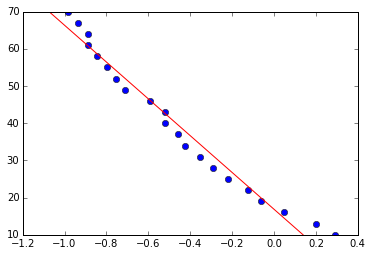
\includegraphics[]{media/lineareregression.png}
\caption{Lineare Regression}
\end{figure}

 So erhalten wir die ausgleichsgerade. Hierauf wenden wir nun die Exponentialfunktion als  Umkehrfunktion an und erhalten so die nichtlineare Kennlinie des Sensors. 
 \begin{figure}[H]
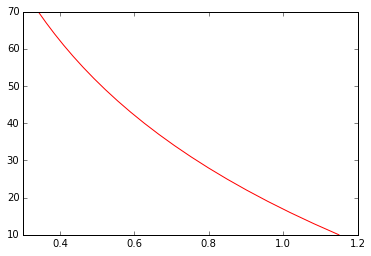
\includegraphics[]{media/finalf.png}
\caption{Kennlinie}
\end{figure}

\begin{figure}[H]
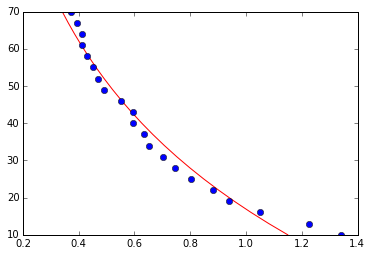
\includegraphics[]{media/messwerte&finalf.png}
\caption{Messwerte und Kennlinie}
\end{figure}

\section{Interpretation}
\label{chap:VERSUCH_2_INTERPRETATION}
Nun haben wir eine Abhängigkeit zwischen Abstand und Spannung geschaffen womit wir den Sensor kalibriert haben. Somit kann der Sensor nun zur Abstandsmessung genutzt werden.
\end{document}